%Preamble:
\documentclass[12pt,onecolumn,letterpaper]{article} %possibilities: book, report, etc
%\documentclass{csuthesis}
%change the fontsize to 12pt, etc if desired
%Also possible \documentclass[10pt,twocolumn]{article}
%Also possible: \documentclass{CSUthesis} (our template)
\linespread{1.5}
%\usepackage[utf8]{inputenc}
%Change margins: Usually taken care of by style file from journal, etc.
\textwidth=6.85in
\oddsidemargin=-0.5in
\textheight=9in
\topmargin=-0.75in

 
\usepackage{breqn}
\usepackage{url,epsfig,graphics,float}
\usepackage{color}
\usepackage{amsmath}
\usepackage{amssymb}
\usepackage{framed}
\usepackage{amsmath}
\usepackage{cite}

\usepackage[inline]{enumitem}
\usepackage[utf8]{inputenc}
\usepackage{dirtytalk}
\usepackage{booktabs}
\usepackage{multirow}
\usepackage{slashbox}
\usepackage{caption,booktabs}


%\usecolortheme[named=UBCblue]{structure}
%\author{Doctoral Candidacy Proposal in Mechanical Engineering} %use \\ to force a line break
%\date{\today} %for no date \date{\empty}
%\title{Dissertation Topic here} %Latex has its own command, and it's case-sensitive
\usepackage[titletoc]{appendix}
\begin{document}
%to suppress page numbering you can use \pagestyle{\empty} (whole doc)
%\maketitle

\begin{titlepage}
\begin{center}

% Upper part of the page. The '~' is needed because \\
% only works if a paragraph has started.
\hfill
\textcolor{blue}{\textbf{\textsc{\Huge DeFiXy Protocol }}}\\
\hfill
\texbf{Support@DeFiXy.com}\\[1.8cm]
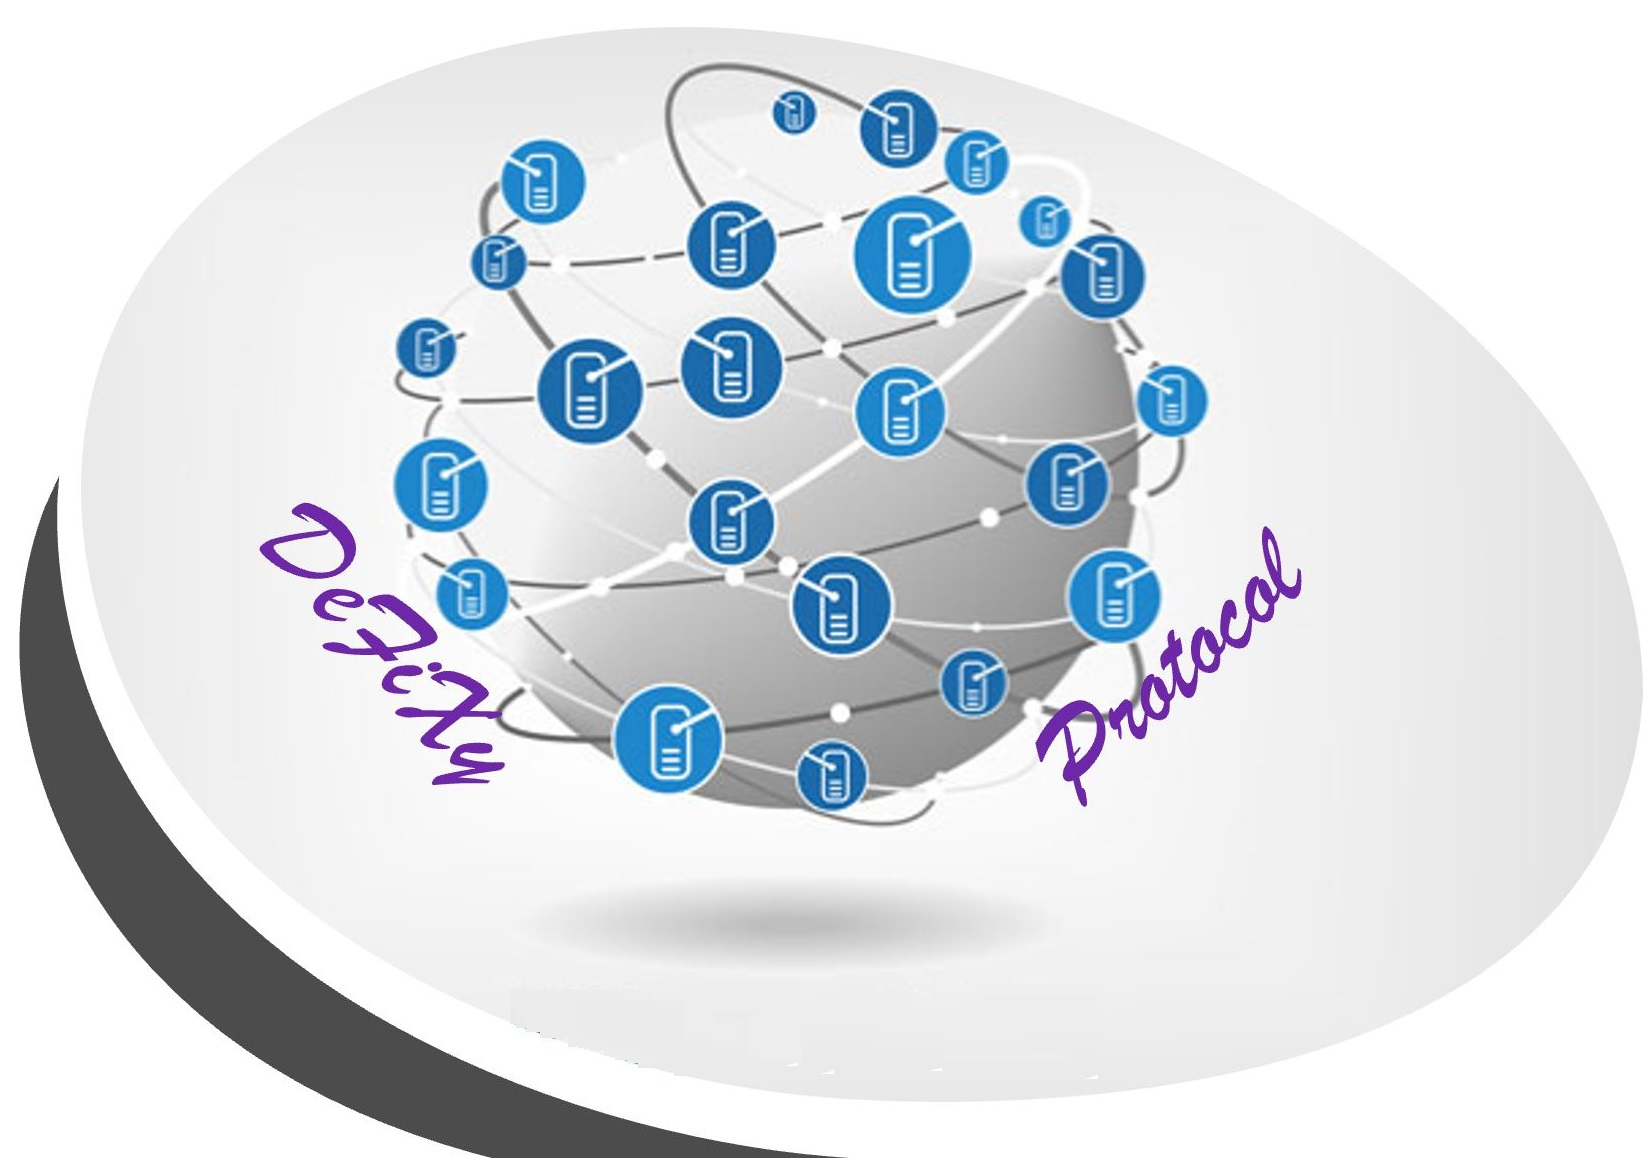
\includegraphics[width=0.5\linewidth]{logo.JPG}
\\[1.8cm]
\hfill
\noindent\rule[0.5ex]{\linewidth}{1pt}
\begin{abstract}
 DeFiXy Protocol is building an amazon-like platform for Crypto Assets. The mission is to actually empower the unbanked by bridging the gap between a fiat-driven economy and the crypto space. This is  indeed a challenge as majority of the unbanked and even the average individual that is interested in venturing into crypto, find it tremendously difficult to transition to using blockchain solutions. DeFiXy Protocol will tackle this challenge by building a user friendly P2P exchange that supports majority of assets and fiats, offer dynamic staking services and decentralized finance services. Our P2P market place will allow users with reputation and collateral to setup their own mini market-place or kiosk where they serve the less experienced users. All the services and features offered by DeFiXy Protocol are integrated in a decentralized manner and allow users enjoy top-notch experience.
 \end{abstract}
\noindent\rule[0.5ex]{\linewidth}{1pt}
\end{center}
\textbf{\small Version: Light Paper 1.0 - May 2020}\\
\textbf{\small This document is prepared by DeFiXy Protocol, it is available for download at DeFiXy.com }
\end{titlepage}
%\tableofcontents
%\listoffigures
%\listoftables

\section{Overview}
This document is DeFiXy Protocol's light paper version 1.0. It contains a surface description of the DeFiXy protocol technology and it's features. A more comprehensive document is under development
\subsection{Problem statment and motivation}
The Blockchain space, as most people know is rapidly growing but due to the complexity that comes with the use of most blockchain solutions like DeFi, the individuals and community of people that are actually in need of the empowerment that comes with blockchain solutions are often left out and are not serviced. We often hear of the saying "blockchain is here to bank the unbanked" or "blockchain is here to empower the unbanked" but the sad truth is that lots of people (the unbanked and even the banked) who should benefit from blockchain solutions are unable to understand and on-board blockchain with ease. Though DeFiXy Protocol is not an educational or onboarding platform for blockchain technologies, it is here to provide a blockchain solution that will actually empower the unbanked and help take the adoption of blockchain technologies one step further into the future.
\subsection{The DeFiXy Protocol}
Simply put, DeFiXy Protocol can be described as an amazon-like blockchain platform which provides an easy to use solution for the everyday crypto-asset user.
\begin{enumerate}
    \item \textbf{P2P market place (exchange):} %Where individuals can trade crypto-assets in a decentralized manner. The main feature of the P2P market-place is the ability for individuals to create mini-kiosk within the platform. Kiosk owners enjoy benefits such as a cut on the transaction fees and other rewards.
    Where individuals can trade crypto-assets in a decentralized manner. The main feature of the P2P market-place are as follows:
\begin{itemize}
\item The ability of users to create trades or setup barter between any pair of whitelisted asset, even between assets that defer in blockchain and also between a whitelisted asset and any of the supported fiats.
\item Individuals with staked assets can create mini-kiosk within the platform, offer customized products and services to other users. Such kiosk owners enjoy a share of the transaction fees accumulated on the platform among other benefits.
\end{itemize}
    \item \textbf{Staking 2.0:} The staking feature offered by DeFiXy protocol provide users with different reward thresholds, these thresholds are functions of two variable, the lockup duration $\tau$ measured in days and the dynamic demand-supply ($\frac{\delta d}{\delta s}(t)$) factor of the asset staked.\\
    The protocol also offers lockup buyout. With this, an individual who initially staked his/her assets for a duration (say 30 days lockup) can unstake prematurely but the action incurs a lockup buyout fee. 
    \item \textbf{DeFi services:} DeFiXy protocol offers DeFi services such as lending and borrowing. users can take out collaterized loans with competitive interest rates. The rates for borrowers and lenders are determined by the users collateral blend ratio ($\beta_r$). \\Since the loans offered do not have maturity period, there are no late payments but the borrower can setup a periodic payment that are deducted automatically in any of the supported assets or fiats as specified by the borrower.\\
    Similarly, a lender can lend asset on a flex period lending mode or on a fixed period lending mode. With the latter offering a better interest rate.
    \item\textbf{Debit card integration:} After meeting the regulatory requirement of target regions, DeFiXy protocol will integrate card payment solutions which will allow users to directly spend crypto assets. 
   \end{enumerate}
DeFiXy protocol will implement all the said features with the average individual with little to no blockchain understanding in mind. The platform will integrate user interface that are highly user-friendly. Individuals will be able to interact with the platform in a smooth and seamless manner, even those that are new to the space.
\newpage
\section{DeFiXy Protocol Token}
\begin{itemize}
    \item \textbf{Token Name:} DeFiXy
    \item \textbf{Token Ticker:} DeFiXy 
     \item \textbf{Token Type:} ERC20
    \end{itemize}
DeFiXy is the native token of the DeFiXy Protocol. It is the utility token that powers DeFiXy protocol. The total supply of this token is limited to 100,000,000 (100 million) and it is pre-mined. The amount of token that will be in circulation at any given time will always be less than or equal to 100 million unless the expansion model is adopted. The circulating supply at the time of main platform launch will be $\approx 15,000,000$ DeFiXy tokens and the maximum supply will be reached in over 10 years from launch.\\
The distribution of DeFiXy is show in Figure~\ref{Chart1}.
   \begin{figure}[h]
\centering 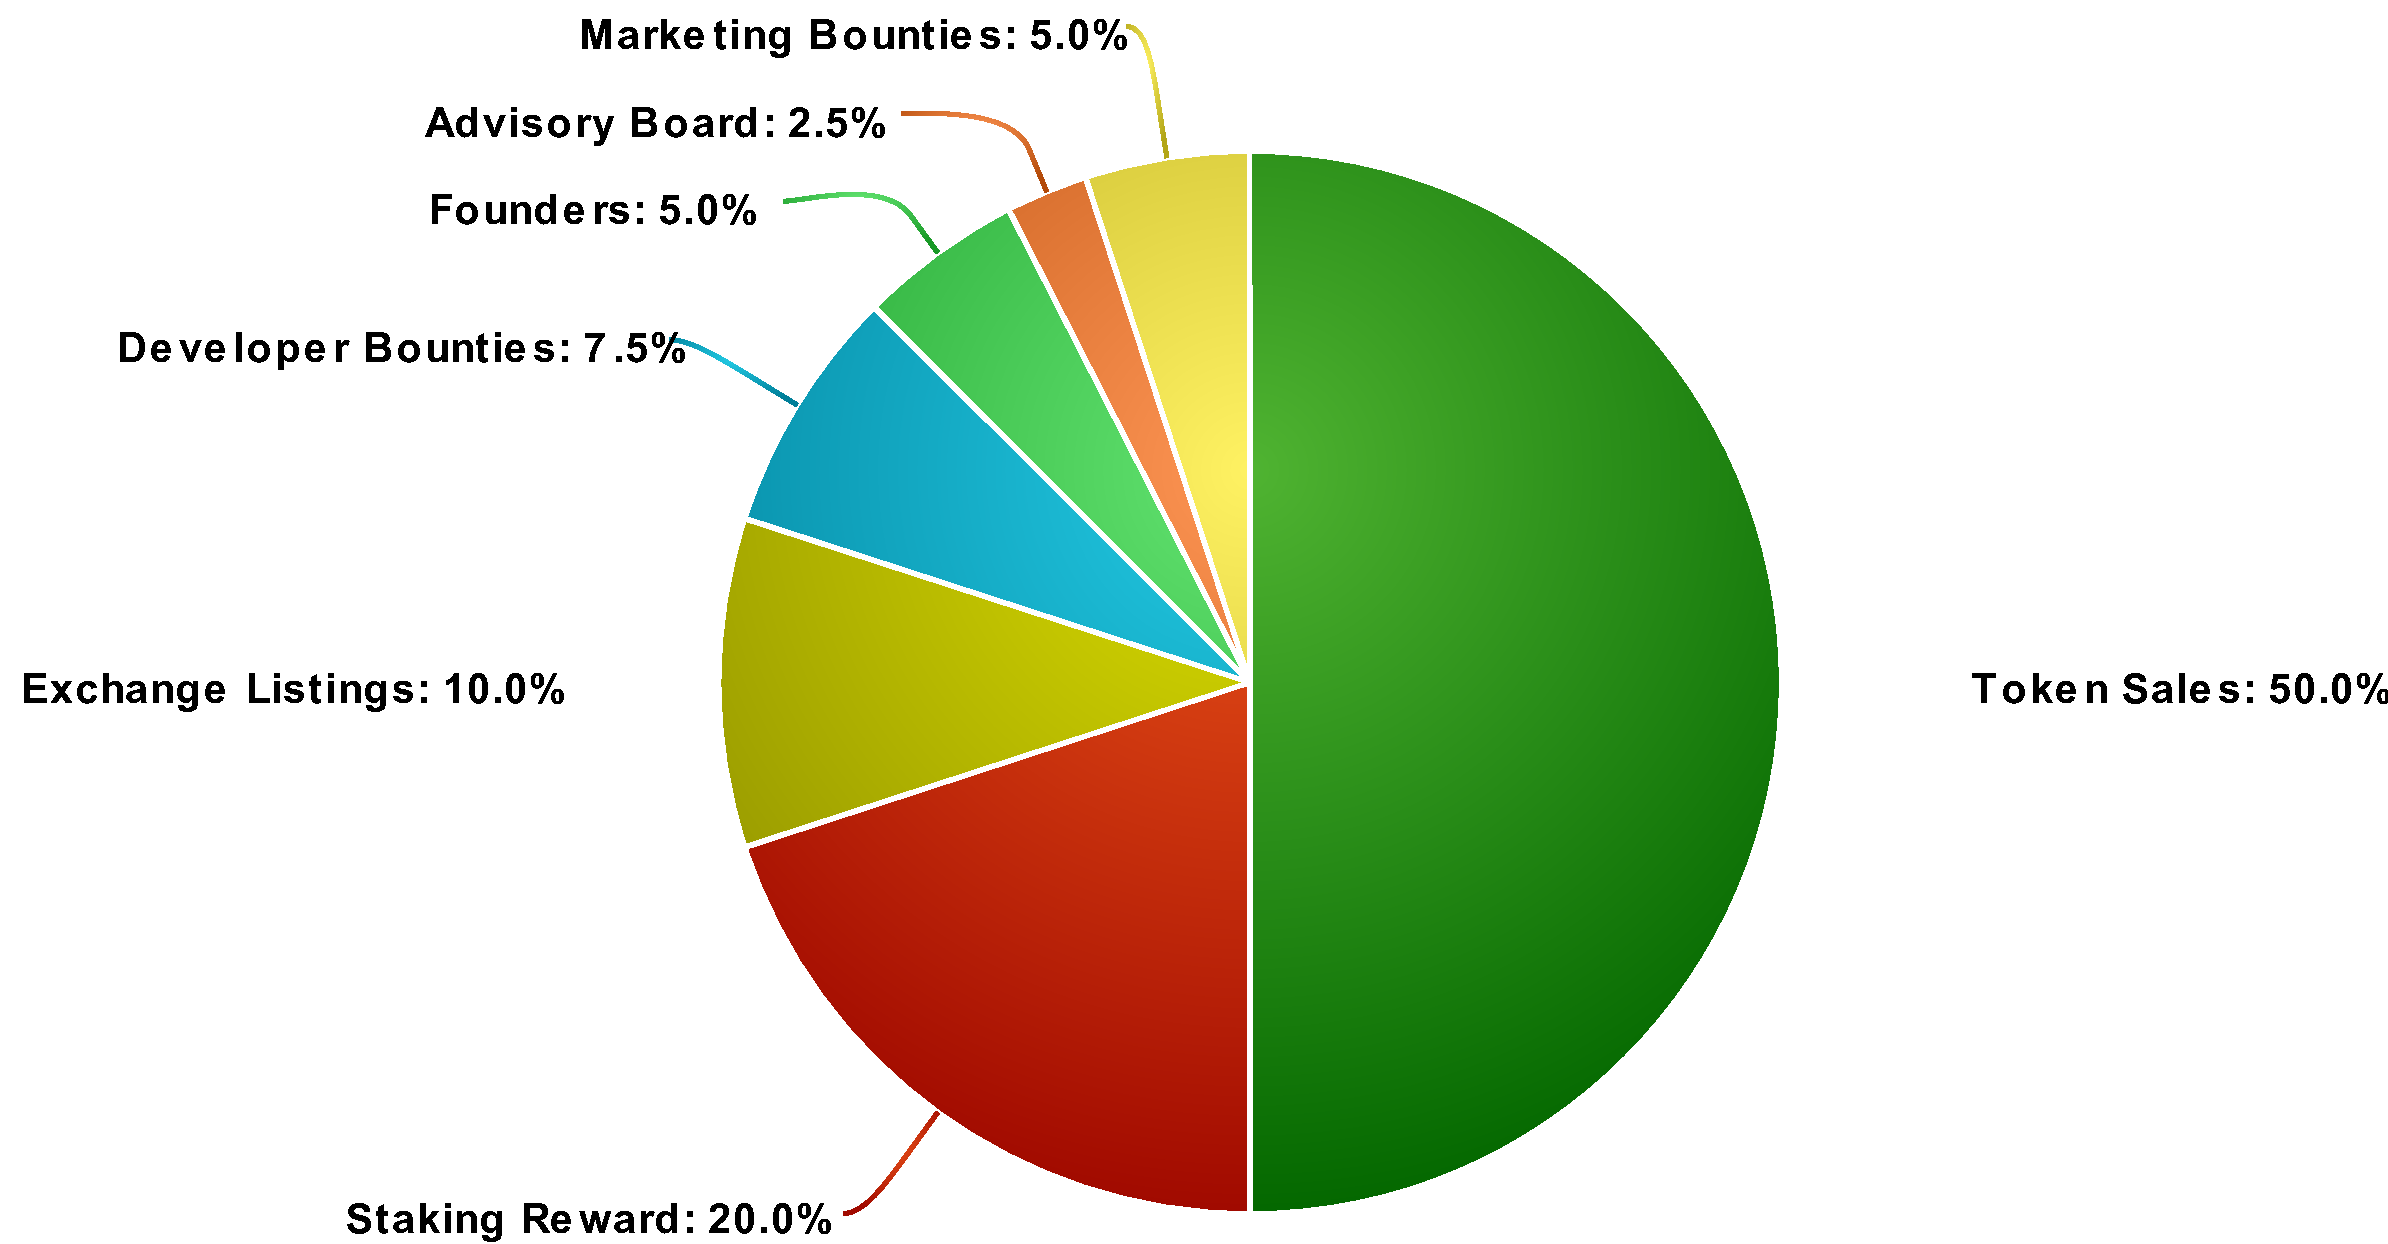
\includegraphics[width=1\linewidth]{Distribution_chart}\caption{DeFiXY distribution at total supply} \label{Chart1}
\end{figure}
  \FloatBarrier
  \newpage
  \subsection{DeFiXy Token Value Proposition}
  As earlier stated, The DeFiXy protocol's token is a utility token that powers DeFiXy protocol. The utility in DeFiXy token and it's value proposition are as follows:
  \begin{enumerate}
    \item \textbf{Mini-Market Categorization Factor $C.F$:}\\
One of the main feature DeFiXy Protocol offer our users is; a platform where p2p trading/bartering can be done freely and at significantly low cost. The cool thing about the p2p market-place is that users also have the option to setup and customize their own mini market-place within the main one. The size of a mini market-place is determined mainly by the size and number of transactions allowable within a given period, this in turn is categorized based on the amount of DeFiXy tokens the mini market-place owner has staked or are delegated to it. \\
A mini market-place that has a large amount of DeFiXy tokens staked/delegated to it will be able to complete more transactions and carry out more trades for other users, hence such a kiosk owner gets a bigger cut of the total transaction fees accumulated on DeFiXy protocol.\\
This is a huge feature, it will help increase the adoption rate of the space. We will be releasing more details on this in the near future.

    \item \textbf{Computation of the Collateral Blend Ratio ($\beta_r$):}\\
    As we can recall, the interest rate of a borrower and the ROI of a lender is heavily dependent on the borrower/lenders collateral blend ratio ($\beta_r$).\\
    A borrower who is holding or staking a large amount of DeFiXy tokens has a larger $\beta_r$ value hence, pays a lower interest rate on loans as compared to one who is holding or staking few amount of DeFiXy tokens.\\
    Similarly, a lender with large amount of DeFiXy tokens held/staked has a higher $\beta_r$ value hence, enjoys a higher return on their investment.
    \item \textbf{Staking Rewards and Transaction Fees:}\\
    Stakers of DeFiXy tokens also get staking rewards in DeFiXy tokens. The fees for transactions carried out on DeFiXy Protocol can also be deducted from a user in DeFiXy tokens. users can decide to have the transaction fees other supported assets but when DeFiXy token is set for transaction fees, the user enjoys a way lower transaction cost.
       \item \textbf{DeFiXy Protocol Asset Pooling Program:}\\
In order to foster growth and rapid adoption of our technology, DeFiXy Protocol will run a periodic asset pooling events  in which users can participate get enormous rewards. The size of pools are capped based on the market expansion need. For user to participate, such a user will pool both DeFiXy token paired with another asset that is part of the list of assets in any particular pooling event.
\end{enumerate}
\section{The Reversible Early Investor Token Sales}
\begin{itemize}
    \item \textbf{Token Name:} 10xDeFiXy
    \item \textbf{Token Ticker:} 10xDF
     \item \textbf{Token Type:} bep8 and ERC20
     \item \textbf{Total Supply:} 2,000,000 10xDF
     \item \textbf{Token sale Starts at:} 8am UTC, Monday 10th of August 2020
     \item \textbf{Token sale Ends at:} 8am UTC, Monday 10th of August 2020
     \item \textbf{sales price:} $\$0.50$ per 10XDF
     \item \textbf{Token swap ratio:} 1 10xDF = 10 DeFiXy
    \end{itemize}
Early investors can participate in our reversible 10X token (10xDF) sale. The token will be sold on Binance dex and uniswap at approximately $\$0.50$. 
10xDF tokens will be swapped for DeFiXy tokens when the platform launches. The swap ratio is set to 1 10xDF = 10 DeFiXy tokens.\\

\textbf{Note} that this is a reversible token sale. As such, participants can reverse their purchases and get back their BNB or ETH (minus transactions fees) as the case may be.\\

Holders will be able to reverse their purchases from the time the token sales ends till the launch of the main platform (latest in December of 2020), at which the tokens can be swapped for DeFiXY tokens.\\

10xDF have a total supply of 2,000,000 (2 million) which is equivalent to 20,000,000 DeFiXy tokens after the swap. 1 million will be sold to early investors on binance dex (bep8 token) and the other 1 million on uniswap (ERC20 token).
\section{Early Investor sales and buy-back Insurance mechanism}
This is how the token sale reversal will work:\\
Each token will sell for approximately $\$0.50$ at initial sales. Though, the 10xDF tokens will continue to trade on exchanges, after the sales are completed, DeFiXy Protocol will place buy orders at the same price at which the tokens were sold. By always having a buy order placed all through the period before platform launch, will allow any early investors to sell their purchased tokens back to DeFiXy Protocol.\\
It should be noted that the 10xDF tokens can be refunded anytime before the lunch of the main platform.\\
This is a way of assuring our early investor, showing that we are committed to the development of DeFiXy protocol.
\section{Money raised utilization}
$100\%$ of money raised, that are not refunded or locked up in the reversal pool, will be spent on bringing talents to the team and on developing DeFiXy protocol.
\newpage
\section*{Reference}
\url{https://github.com/ethereum/wiki/wiki/White-Paper}\\
\url{https://www.ampleforth.org/basics/}
\url{https://www.orionprotocol.io/}\\
\url{https://tixl.me/whitepaper/}\\
\url{https://pamp.network/}

\end{document}